\documentclass[tikz,border=8pt]{standalone}
\usepackage{amsmath,amssymb}
\usetikzlibrary{arrows.meta,calc,decorations.pathmorphing}

\begin{document}
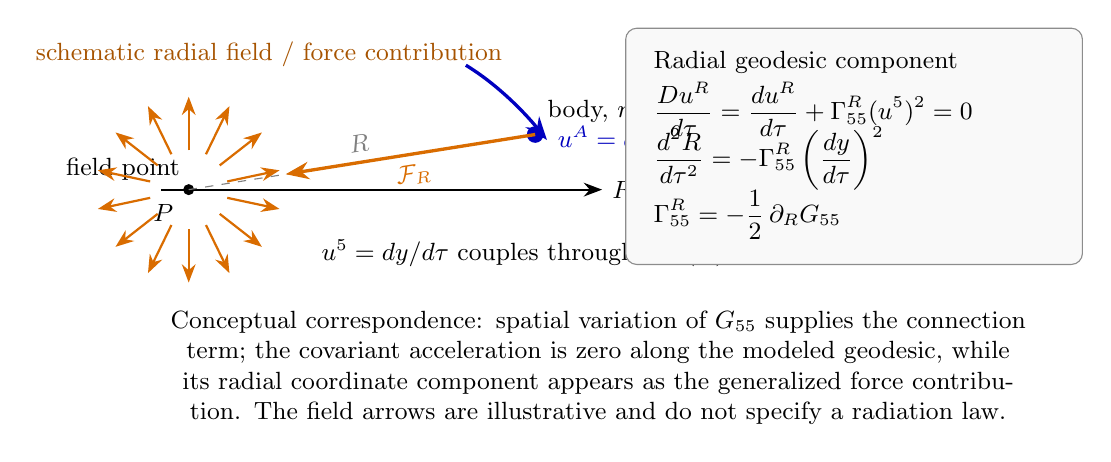
\begin{tikzpicture}[
    >=Stealth,
    font=\small,
    axis/.style={->,thick},
    field/.style={->,thick,orange!85!black},
    path/.style={->,very thick,blue!75!black},
    note/.style={align=center,inner sep=3pt}
]
    % Spatial sketch: a point P and a moving body at radius R.
    \coordinate (P) at (0,0);
    \coordinate (B) at (4.4,0.7);
    \draw[axis] (-0.35,0) -- (5.25,0) node[right] {$R$};
    \fill[black] (P) circle (2pt);
    \node[below left=2pt] at (P) {$P$};
    \node[note,above left] at (P) {field point};

    % Schematic radial field arrows around P.
    \foreach \ang in {12,38,64,90,116,142,168,-12,-38,-64,-90,-116,-142,-168} {
        \draw[field] ($(P)+(\ang:0.5)$) -- ($(P)+(\ang:1.18)$);
    }
    \node[note,orange!65!black] at (1.02,1.72) {schematic radial field / force contribution};

    % Body position and its trajectory; radial direction from P is explicit.
    \draw[gray,dashed] (P) -- (B) node[midway,above,sloped] {$R$};
    \fill[blue!75!black] (B) circle (3pt);
    \node[above right=1pt] at (B) {body, $m$};
    \draw[path] (3.52,1.58) .. controls (3.9,1.35) and (4.25,1.0) .. (4.55,0.63)
        node[right] {$u^A = dx^A/d\tau$};
    \draw[field,very thick] (B) -- ($(B)!0.72!(P)$)
        node[midway,below,sloped] {$\mathcal{F}_R$};
    \node[note,below] at (4.25,-0.52) {$u^5=dy/d\tau$ couples through $G_{55}(R)$};

    % Covariant-derivative correspondence.
    \draw[rounded corners,draw=black!45,fill=gray!5] (5.55,-0.95) rectangle (11.35,2.05);
    \node[anchor=west,align=left] at (5.78,1.62) {Radial geodesic component};
    \node[anchor=west] at (5.78,1.02)
        {$\displaystyle \frac{D u^R}{d\tau}
          =\frac{d u^R}{d\tau}+\Gamma^R_{55}(u^5)^2=0$};
    \node[anchor=west] at (5.78,0.40)
        {$\displaystyle \frac{d^2R}{d\tau^2}
          =-\Gamma^R_{55}\left(\frac{dy}{d\tau}\right)^2$};
    \node[anchor=west] at (5.78,-0.32)
        {$\displaystyle \Gamma^R_{55}=-\frac{1}{2}\,\partial_R G_{55}$};

    \node[below,align=center,text width=11cm] at (5.2,-1.42)
        {Conceptual correspondence: spatial variation of $G_{55}$ supplies the connection term;
        the covariant acceleration is zero along the modeled geodesic, while its radial
        coordinate component appears as the generalized force contribution. The field arrows
        are illustrative and do not specify a radiation law.};
\end{tikzpicture}
\end{document}
